\section{Introduction}
\label{introduction}

Fine-tuning is an effective method for specializing large pre-trained models, either by using direct supervision from the training set of a given task \citep{ruder_18, devlin_19, raffel_20}, from curated instruction datasets \citep{DBLP:conf/acl/MishraKBH22, wei_22, alpaca}, or from human feedback via reinforcement learning \citep{ouyang_22, bai_22, touvron_23}. 
However, fine-tuning is not necessarily an efficient method,
especially for transformer-based large language models (LLMs),
since their large number of parameters leads to large compute and memory requirements.
For instance, fine-tuning GPT-3 175B~\citep{DBLP:conf/nips/BrownMRSKDNSSAA20} or LLama 65B~\citep{touvron_23} 
typically requires 1,200 GB and 780 GB of GPU memory, as reported in \citet{hu_22} and \citet{dettmers_23}, respectively.

 \begin{figure}[t]
\centering
 	\makebox[0.4\textwidth][c]{
 		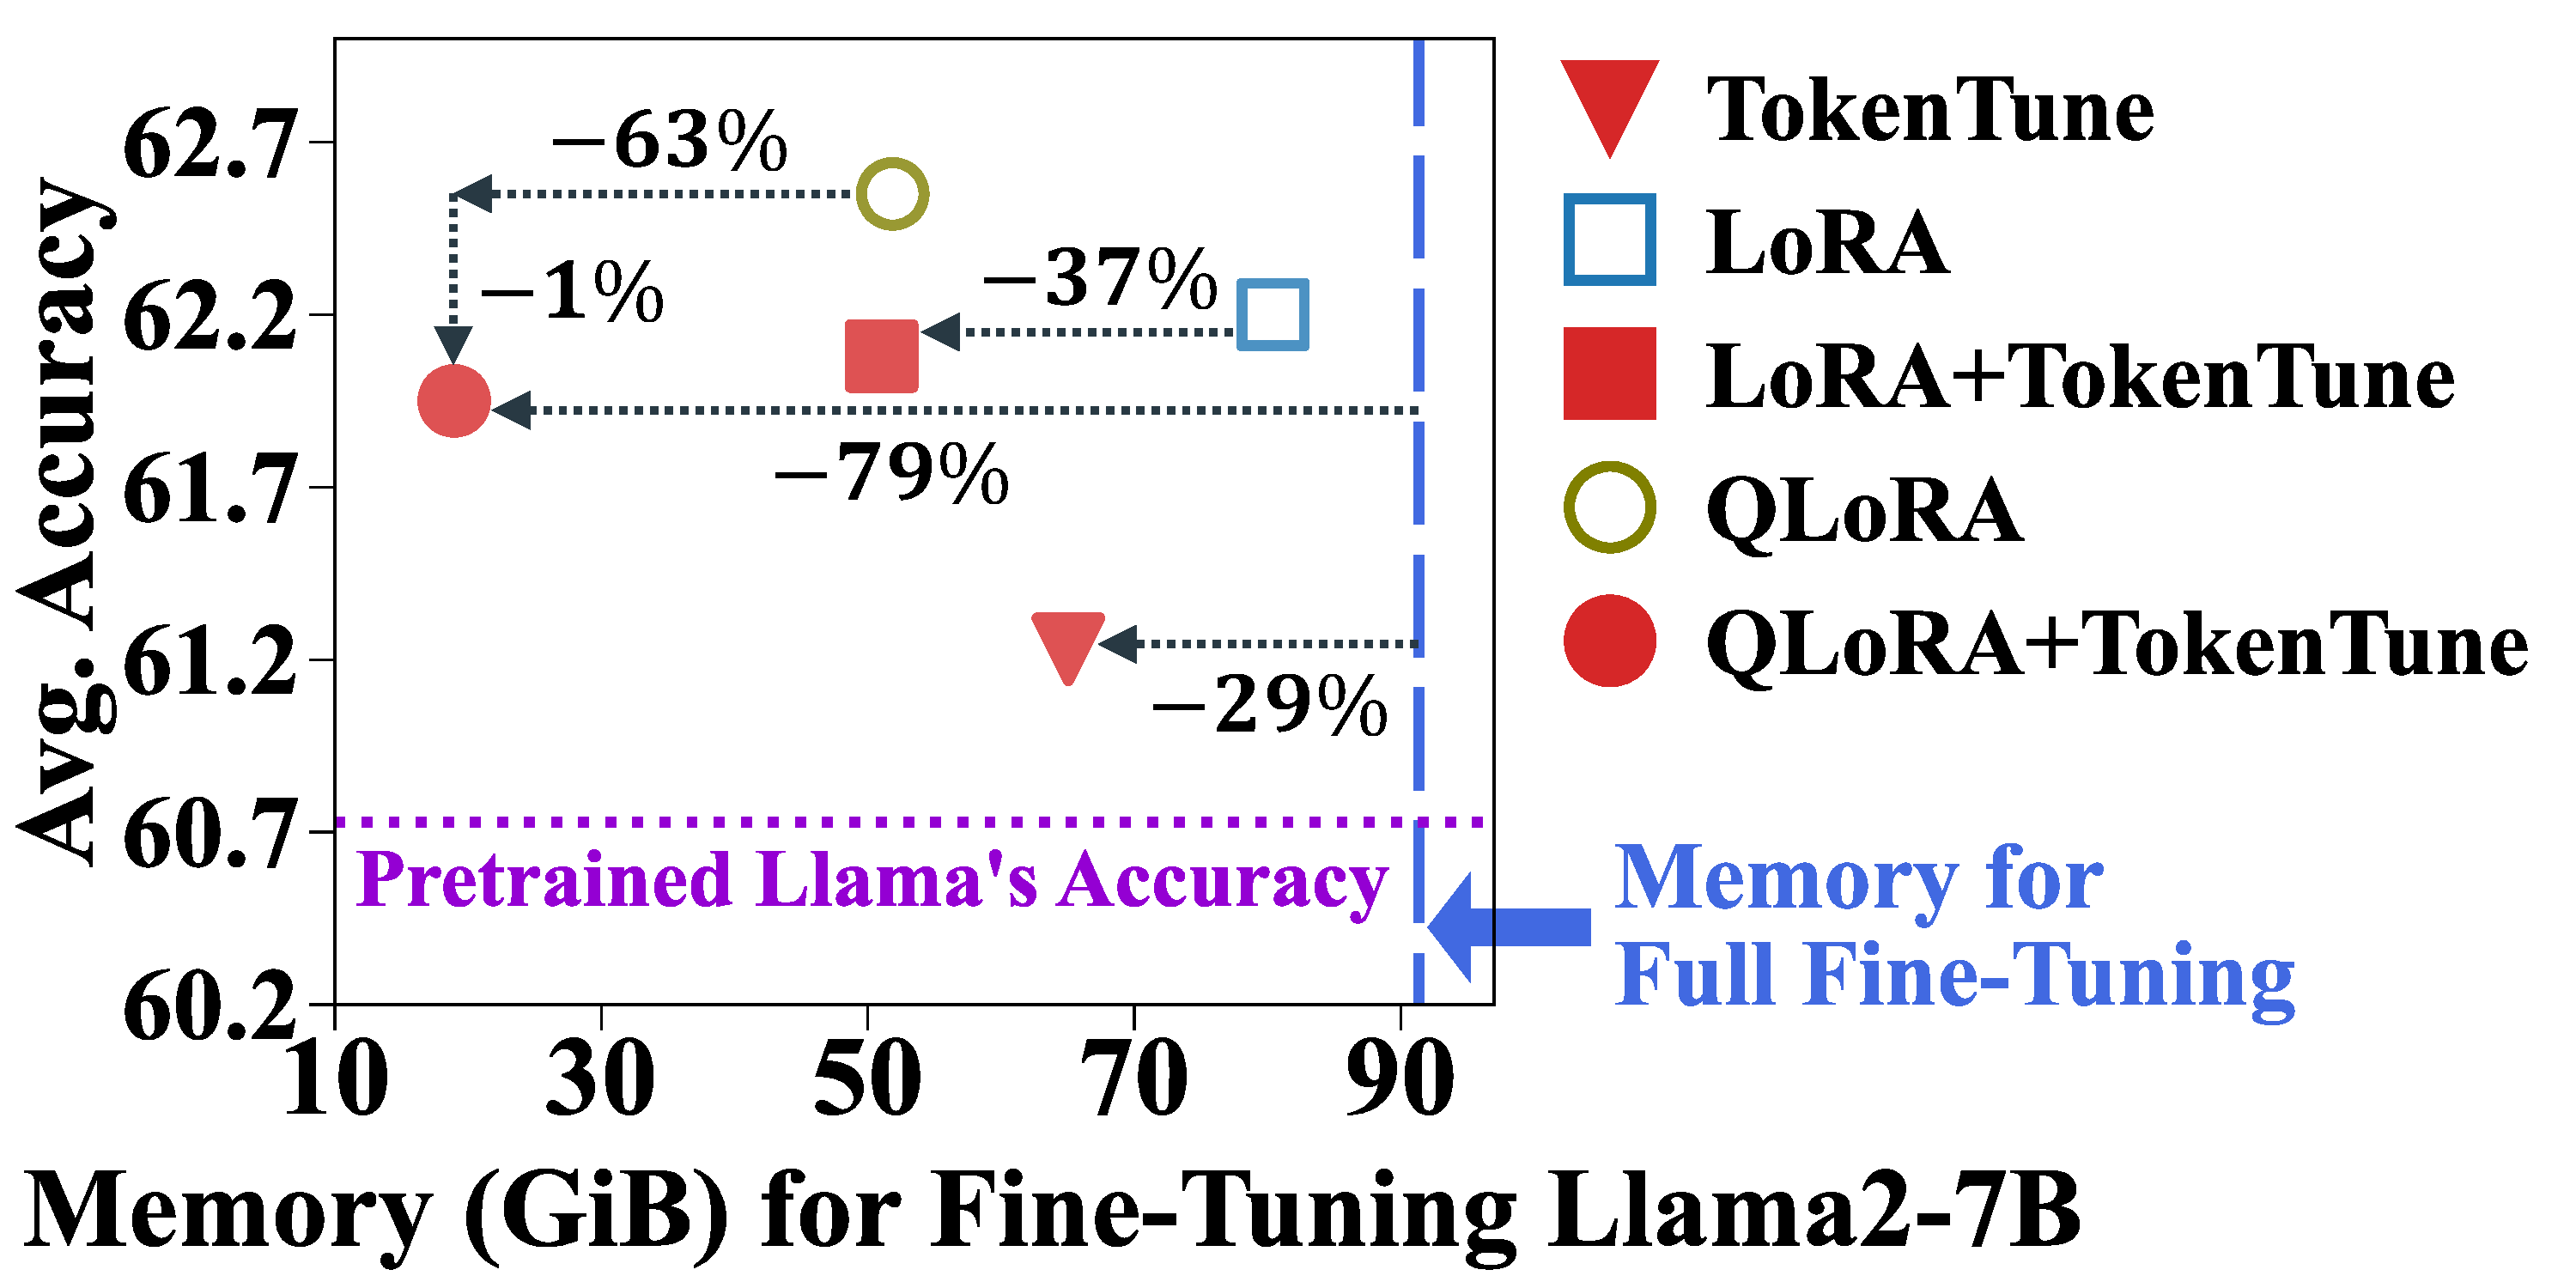
\includegraphics[width=1.02\columnwidth]{figures/crown_jewel_annotated.pdf}
 	}
\caption{\method greatly \mbox{reduces} the GPU memory usage for fine-tuning the \mbox{Llama2-7B} model 
(e.g., using only 37\% of the memory~QLoRA~\citep{dettmers_23} requires),
while achieving similar accuracy to representative memory-efficient fine-tuning methods.
 		Accuracy and memory usage numbers are listed in \Cref{tab:llm-perf} and Fig.~\ref{fig:llm-memory}.
 		See Sec.~\ref{sec:exp:large} for details on experiments.
 	}
 	\label{fig:crownjewel}
 \end{figure}


GPU memory usage during fine-tuning can be broken down into three parts: 
storing (1) the model parameters, (2) the parameter gradients and optimizer states, and (3) the intermediate activations. 
Parameter-Efficient Fine-Tuning (PEFT)~\citep{DBLP:conf/icml/HoulsbyGJMLGAG19, hu_22} aims at updating a small number of parameters, 
e.g., by optimizing a subset of the backbone model's parameters while freezing others,
which reduces the memory requirements to store the parameters' gradients and optimizer states.
Alternatively, quantization techniques~\citep{dettmers_22, dettmers_23, liu_23} use low precision data types for model parameters, which reduces the memory cost.
For example, in fine-tuning the Llama2-7B model,
LoRA~\citep{hu_22} and QLoRA~\citep{dettmers_23}, which are representative PEFT and quantization-based methods,
reduce the memory needed for full fine-tuning by 12\% and 43\%, respectively (\Cref{fig:crownjewel}).
However, such existing approaches still require caching all of the intermediate activations computed in the forward pass
to obtain the gradients during the backward pass.







In this work, we propose a method for memory-efficient fine-tuning, named \method, 
which aims to significantly reduce the GPU memory dedicated to storing intermediate activations during the forward pass
without sacrificing the model performance on various downstream tasks.
To this end, \method selects a subset of the input tokens in the context, and fine-tunes the model with respect to those selected tokens.
More specifically, during the backward pass, \method approximates the gradient computation by backpropagating through the selected tokens, and thus 
only a subset of the intermediate activations need to be cached during the forward pass, thereby reducing the memory cost.

We demonstrate the effectiveness of \method using both medium- and large-size language models, namely, BERT~\citep{devlin_19} and Llama~\citep{touvron_23}, 
which have hundreds of millions, and billions of parameters, respectively.
Overall, our results show that fine-tuning with \method leads to downstream task performance on par with that of full fine-tuning or representative methods for memory-efficient fine-tuning,
while drastically reducing the memory footprint.
Notably, \method can be effectively combined with existing methods, achieving a greater reduction in memory usage.
For instance, by combining \method with QLoRA~\citep{dettmers_23}, 
we can fine-tune Llama2-7B using just about one third of the memory QLoRA alone requires as \Cref{fig:crownjewel} shows.
To~sum, our contributions are as follows.
\begin{itemize}[leftmargin=1em,topsep=-2pt,itemsep=-3pt]
	\item \textbf{Novelty.} \method, to the best of our knowledge, is the first method that reduces GPU memory usage for fine-tuning via token selection\footnote{A preliminary version of this work was presented at a non-archival workshop~\citep{simoulin2023memoryefficient}.}.
	\item \textbf{Combinability.} \method can be combined with existing memory-efficient fine-tuning methods, leading to further memory reduction.
	\item \textbf{Effectiveness.} We perform extensive experiments, showing that 
	\method achieves similar accuracy to representative memory-efficient methods,
	while greatly reducing the memory footprint during fine-tuning,
	e.g., using only 21\% of what full fine-tuning requires (\Cref{fig:crownjewel}).
\end{itemize}










